% Completed TRAIN findings; frozen evaluation fragments are included below.
\section{Experiments}
\label{sec:experiments}

We distinguish representability, scalar fit and scheduling performance.
All conditions share the typed library and classical kernel; shared-search
gains alone do not establish LLM-guidance benefit.

\subsection{Decision Evidence and Authoring Design}
TRAIN contains 120 unit-weight states with at most 32 vertices: 24
source-induced public graphs and 96 contact endpoints forming 48 intervention
pairs. Public clusters are partitioned within a previously exposed corpus.
Contact pairs preserve opportunities and change only ground switching gap,
$0\!\to\!1$; satellite gap remains zero and capacities one.
Queries precede certification and retain shortfalls. Of 1,503 comparisons,
594 are strict, 909 tie and none are unknown; 90 strict comparisons alias
under base-nine vectors. Among 630 paired queries, 12 reverse and 123
preserve strict preferences, 294 tie on both sides and 201 have one tied
endpoint. This controlled,
alias-enriched frame diagnoses conflicts, not their natural incidence.

R2 repairs a shared rejected interface and cycle. Prompts show six cases and
eleven relations; checking retains all 594 requirements. Five blocks contain
eight proposals per W/R/O arm; the first four form the preregistered matched
cohort and the fifth remains reported. Authoring requests
\texttt{gpt-6.1-sol}/ultra; the served backend is undisclosed.
All 120 programs complete server TRAIN assessment with feasible incumbents.
Matched slots do not match compute.

\subsection{What Witness Feedback Repairs}
Matched information-gate yield is 26/32 W versus 19/32 R, a 21.875-point
difference (Table~\ref{tab:v06-authoring}). The table also retains the complete
five-block cohort; Figure~\ref{fig:v06-yield} plots all five bank counts per
arm against measured author-call wall cost.
These are conditional interface repair findings, not general model efficacy.

\begin{table}[t]
\centering
\fontsize{9}{10.4}\selectfont
\setlength{\tabcolsep}{3pt}
\caption{R2 information-gate yield: eligible/original positions in all five
blocks and the preregistered matched four. Bold marks observed column bests.}
\label{tab:v06-authoring}
\begin{tabular}{lrr}
\toprule
Arm & All five & Matched four\\
\midrule
\textbf{W} & \textbf{28/40} & \textbf{26/32}\\
R & 24/40 & 19/32\\
O & 0/40 & 0/32\\
\bottomrule
\end{tabular}
\end{table}
\begin{figure}[t]
\centering
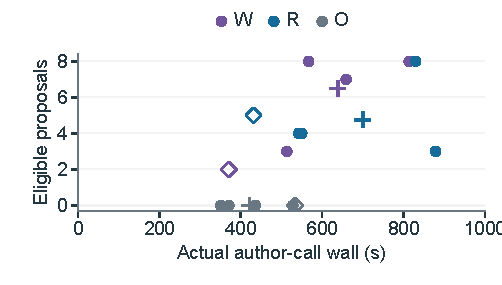
\includegraphics[width=.92\columnwidth]{figures/refinement_authoring_efficiency_v06.pdf}
\Description{Gate-eligible proposals and measured author-call wall time for all five banks in every arm. The fifth bank is distinguished rather than removed.}
\caption{LLM proposal efficiency: eligible proposals versus actual
author-call wall time. All five banks remain shown; the fifth is hollow
and matched means are crosses. Times describe whole calls.}
\label{fig:v06-yield}
\end{figure}

Matched W/R banks produce 10.18/6.78 eligible proposals per 1,000 measured
author-call seconds, descriptively conditional on this seed and these calls.
The gate measures whether the demanded features admit a consistent ordering;
it does not certify the authored scalar or scheduling benefit. Detailed scalar
fit, feature work and policy quality remain in the supporting report and
Discussion, separate from information repair.
All TRAIN schedule qualities equal $2693/4480$ under Eq.~\ref{eq:train-macro-quality};
there is no observed TRAIN reward improvement, before any distribution shift.

Deployment freezes four genuine W joint and twelve matched quality-only
selections before TEST certification; evaluation outcomes select no winner.
Joint-versus-quality contrasts include selection, not isolated witness effects.

\subsection{Complete Quotient Checking and Feature Cost}
The optional catalogue contains all 53 canonical expressions from valid
cold authoring, adaptively discovered on TRAIN, with the same 594 requirements
and $K=6$. Its 4/8/16-expression prefixes remain cyclic. The full catalogue
resolves the quotient using four features at exact minimum additive cost
1,371,468; a verified nonnegative weighting of necessary cuts proves the
matching lower bound.

Seven self-loop cuts precede two cycle cuts: removing self-loops leaves a
cycle, and splitting it exposes another, requiring the ninth full-inventory
check (Figure~\ref{fig:v06-catalogue}). Greedy tie orders remain
identifier-sensitive. This certifies scoped representation repair and an
additive feature-work proxy, not a fitted scalar or runtime optimum.

\begin{figure*}[t]
\centering
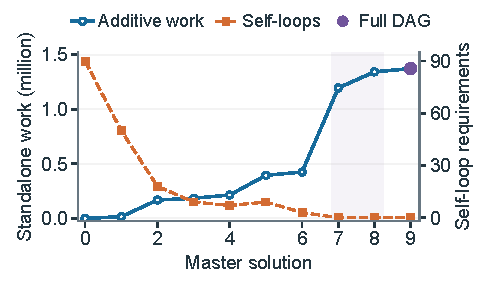
\includegraphics[width=.45\textwidth]{figures/refinement_cost_curve_v06.pdf}\hfill
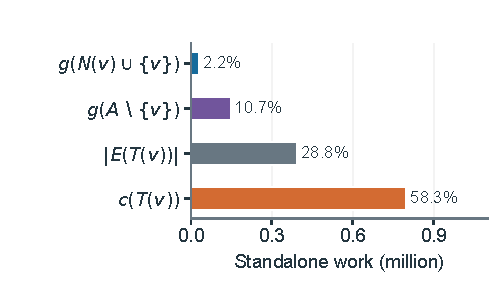
\includegraphics[width=.45\textwidth]{figures/refinement_feature_work_v06.pdf}
\Description{Full-quotient obstructions and additive feature work across catalogue trials; work composition of the certified four-feature minimum.}
\caption{TRAIN catalogue repair: full-quotient obstructions and additive
cost (left), minimum-cost feature work (right). Cyclic trials are not repairs.
Standalone work excludes shared-DAG savings and complete-policy cost.
$g(S)$ is greedy-packing weight, $T(v)=A\setminus(\{v\}\cup N(v))$,
and $c(S)$ is clique-cover upper-bound weight.}
\label{fig:v06-catalogue}
\end{figure*}

\subsection{Published Solvers and Common Components}
Stochastic native solvers use three fixed seeds; deterministic methods and
Degree use one. Exact transformations preserve objectives; signed-range
incompatibilities remain nulls. Coverage and actual costs accompany rewards;
nominal targets are not end-to-end hard deadlines.

EoH-DSL~\cite{liu2024eoh} adapts published operators in four runs of eight
genuine calls with a two-member distinct-quality population. The typed interface
and common rejected seed delimit this reproduction. Its four frozen deployment
identities retain the shared seed; full TRAIN fitness and authoring cost are
reported in the supporting material and Discussion. Authoring compute is not
matched to R2.

\subsection{Adaptation to Withheld Constraint Configurations}
\label{sec:v06-heldout}

\begin{figure*}[!t]
\centering
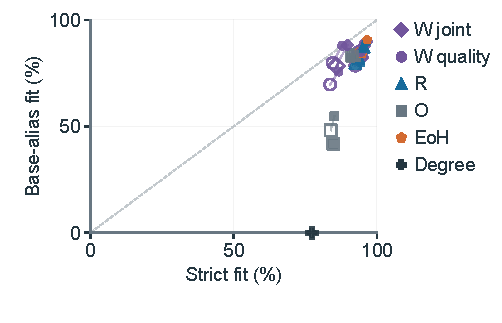
\includegraphics[width=.45\textwidth]{figures/heldout_strict_alias_movement_v06.pdf}\hfill
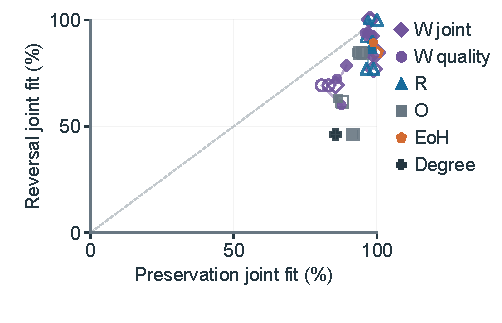
\includegraphics[width=.45\textwidth]{figures/heldout_pair_joint_movement_v06.pdf}
\Description{Strict versus base-alias scalar fit and strict-preservation versus strict-reversal joint correctness for the 21 predeclared main identities. Hollow points are original observations; solid points are the complete five-rename means, with thin connectors retaining movement.}
\caption{Frozen preference transfer: strict versus base-alias fit (left),
strict-preservation versus strict-reversal correctness (right). Hollow/solid
points denote original/five-rename means of all 21 predeclared identities;
coincident identities and renamings remain dependent.}
\label{fig:v06-heldout}
\end{figure*}

The mechanism TEST contains 24 source-disjoint public states and 48 newly
drawn contact endpoints forming 24 pairs. Contact generation retains TRAIN's
resource regimes and unit weights, but uses new seeds and withheld gaps
$0.25\!\to\!2$. Within a pair, the same contacts induce two conflict graphs.
All four W-joint rules omit the available gap coordinates and recompute
structural features from the current graph. No TEST preference label enters
their scoring. Certification occurs after the program
freeze and supplies evaluation targets only.

We evaluate 31 frozen identities and five prescribed identifier renamings.
Of 962 comparisons, 453 are strict (including 79
base-nine aliases) and 509 are exact ties. The 355 paired queries comprise
13 strict reversals, 83 strict preservations, 130 ties on both endpoints and
129 with one tied endpoint. All 190 quota shortfalls remain recorded.
Programs and selections freeze before evaluation certification; no TEST
outcome selects a winner.

Across four blocks, W joint attains mean original strict/base-alias fit of
91.94/81.96\%. Its strict advantage over W quality is 3.37 percentage points
(source-cluster 95\% interval: 2.04--4.72).
Joint-versus-quality comparisons include selection; intervals condition on
the frozen programs, not model-population effects. All four original demanded
feature quotients are acyclic. This evaluates scoped information repair and
actual scalar fit separately.

Both endpoints must satisfy their certified strict requirements for paired
correctness. Mean W joint reversal/preservation correctness is
82.69/95.48\% (Table~\ref{tab:v06-paired-adaptation}). These targets concern
configuration response, rather than arbitrary public-graph rankings.
Figure~\ref{fig:v06-heldout} retains every predeclared main
identity and its complete five-rename mean; no outcome selects plotted
programs. Renaming is a separate stress test, not an invariance guarantee.
The four EoH identities retain their seed origin and remain dependent.

\begin{table}[!t]
  \centering
  \caption{Ranking adaptation to gap $0.25\!\to\!2$ with identical contacts:
  all 13 reversal and 83 preservation requirements, original mapping.
  LLM rows average four dependent frozen outputs; Degree has one.
  EoH~\cite{liu2024eoh} retains a shared seed AST. Counts are output--requirement
  positions, not independent sources or scheduling gains.}
  \label{tab:v06-paired-adaptation}
  \setlength{\tabcolsep}{4pt}
  \begin{tabular}{lrr}
  \toprule
  Frozen cohort & Reversal (\%) & Preservation (\%) \\
  \midrule
  W joint & 82.69 (43/52) & 95.48 (317/332) \\
  W quality & 82.69 (43/52) & 89.76 (298/332) \\
  R quality & \textbf{86.54} (45/52) & 97.89 (325/332) \\
  O quality & 69.23 (36/52) & 92.17 (306/332) \\
  EoH-DSL & 84.62 (44/52) & \textbf{100.00} (332/332) \\
  Degree & 46.15 (6/13) & 85.54 (71/83) \\
  \bottomrule
  \end{tabular}
\end{table}


All 13,392 shared-kernel assignments complete with feasible incumbents.
The supporting report retains all 31 identities, full cohort contrasts,
renaming obstructions, rewards and measured costs; Discussion examines their
limits. These transfer measures characterize information repair; scheduling
quality is assessed separately.


\begin{table*}[!t]
\centering
\small
\setlength{\tabcolsep}{3pt}
\caption{Published solvers and frozen deployment at nominal $T=5$: within-family mean objective and measured standalone CPU seconds. WDP objectives are displayed in millions. Superscripts mark defined/assigned contexts; a partial reward mean cannot establish superiority over a fully covered method. Unsupported native executions have no displayed cost; other costs include failed attempts, charged initialization and repair, with graph loading separate. Bold marks lowest observed mean CPU among fully covered methods. All 13 families and targets remain in the report.}
\label{tab:v06-published}
\begin{tabular}{lrrrrrrrr}
\toprule
Method & \multicolumn{2}{c}{Standard/balanced} & \multicolumn{2}{c}{Dense/ground} & \multicolumn{2}{c}{WDP 4xx} & \multicolumn{2}{c}{Grids}\\
 & $w(I)$ & CPU & $w(I)$ & CPU & $w(I)/10^6$ & CPU & $w(I)$ & CPU\\
\midrule
CHILS~\cite{grossmann2025chils} & 7,277.9 & 5.01 & 978.2 & 5.08 & 75.5735 & 5.17 & 59,093.5 & 5.05\\
ILS~\cite{grossmann2025chils} & 7,277.9 & 5.02 & 978.2 & 5.09 & 75.5735 & 5.23 & 59,039.6 & 5.06\\
M$^2$WIS~\cite{grossmann2024mmwis} & 7,277.9 & 0.19 & 978.2 & 1.01 & ---$^{0/6}$ & --- & ---$^{0/10}$ & ---\\
Struction~\cite{gellner2021struction} & 7,277.9 & 0.03 & 978.2 & \textbf{0.21} & ---$^{0/6}$ & --- & ---$^{0/10}$ & ---\\
WeightedBR~\cite{lamm2019weighted} & 7,277.9 & \textbf{0.02} & 977.5 & 3.59 & ---$^{0/6}$ & --- & ---$^{0/10}$ & ---\\
Degree / CHILS & 7,277.9 & 3.30 & 978.2 & 3.56 & 75.5735 & \textbf{2.81} & 59,077.4 & \textbf{4.75}\\
EoH / CHILS~\cite{liu2024eoh} & 7,277.9 & 3.88 & 978.2 & 4.88 & 75.5735 & 3.12 & 59,077.4 & 4.96\\
Joint W / CHILS & 7,277.9 & 4.25 & 978.2 & 5.03 & 75.7194$^{5/6}$ & 3.29 & ---$^{0/10}$ & 4.45\\
\bottomrule
\end{tabular}
\end{table*}

\IfFileExists{figures/performance_cpu_scaling_v06__fresh_standard_balanced__standard_balanced.pdf}{%
\begin{figure*}[!t]
  \centering
  \begin{minipage}[t]{0.495\textwidth}
    \centering
    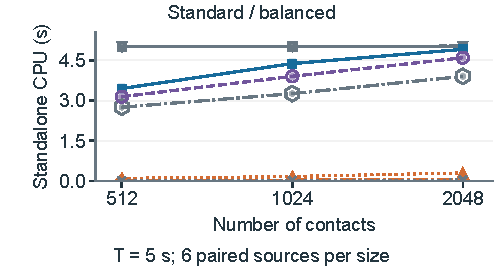
\includegraphics[width=\linewidth]{figures/performance_cpu_scaling_v06__fresh_standard_balanced__standard_balanced.pdf}
    {\small (a)}
  \end{minipage}\hfill
  \begin{minipage}[t]{0.495\textwidth}
    \centering
    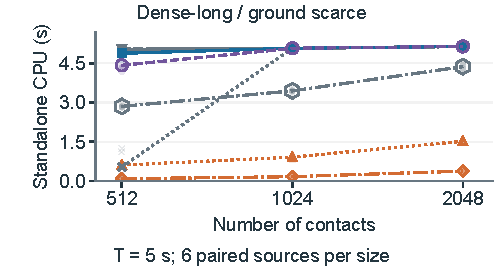
\includegraphics[width=\linewidth]{figures/performance_cpu_scaling_v06__fresh_dense_long_ground_scarce__dense_long_ground_scarce.pdf}
    {\small (b)}
  \end{minipage}
  \par\vspace{1pt}
  
\includegraphics[width=\textwidth]{figures/performance_cpu_scaling_legend_v06.pdf}
  \caption{Measured deployment CPU versus contact count at fixed nominal
  $T=5$ seconds: standard balanced (a) and dense-long ground scarce (b).
  Faint points show six paired sources per size; lines show their mean,
  after within-context seed/member averaging. Warm policies each charge
  the full common CHILS initializer and their own repair; shared graph
  loading remains separate. These are scale comparisons, not anytime traces
  or evidence of LLM speed superiority. Complete gain/coverage matrices
  remain in the supporting report.}
  \Description{Two panels compare actual standalone CPU seconds at contact
  counts 512, 1024, and 2048 for five native method families and warm
  joint witness, EoH-DSL, and Degree policies. Each faint point is one
  paired-source cost; each line joins the six-source means at the three
  sizes. All policies use their frozen identities and native methods
  retain their prescribed seeds. A shared legend identifies eight curves.
  The comparison uses fixed nominal five-second targets and retains
  the full charged common initializer for warm policies.}
  \label{fig:v06_performance_budget}
\end{figure*}
}{}

\subsection{From Full-Residual Evidence to Restricted Patches}
\label{sec:v06-patch-bridge}
A TRAIN bridge examines first patches of 120 common-Degree traces;
106 contain only two vertices. Degree fits all 15 local strict labels;
W joint fits 58/60 output--label positions. Of seven full-strict pairs,
one reverses and three tie under the outside-fixed patch boundary.
Thus full-residual fit cannot certify patch preference or search efficiency.
Complete rows, comparator fits and shortfalls remain in the report.

\subsection{Published-Solver Comparison and Joint-Shift Stress}
\label{sec:v06_performance}

We evaluate all 23 frozen policy identities on 302 contexts at nominal wall
 targets $T\in\{0.1,1,5\}$ seconds. Newly drawn scheduling problems provide
216 endpoints from 108 resource-intervention pairs. Public inputs comprise
25 WDP, three Segmentation, and ten Grids sources from the weighted-clique
benchmark~\cite{mccreesh2017evaluation}, retaining exact weights and complement
orientation. Public source clusters follow fixed withholding within previously
exposed corpora. Two 24-context C3 tracks remain separate exploratory analyses.

Table~\ref{tab:v06-published} displays four predeclared families at $T=5$
against CHILS and ILS~\cite{grossmann2025chils}, M2WIS~\cite{grossmann2024mmwis},
Struction~\cite{gellner2021struction}, and WeightedBR~\cite{lamm2019weighted}.
The deployment comparison keeps the same strong CHILS incumbent and repair
limits for joint witness, Degree, and EoH-DSL policies. Four frozen EoH-DSL
outputs retain their common seed AST~\cite{liu2024eoh}. Every warm policy is
charged the full shared initializer and its own repair cost; nominal targets
are not equal end-to-end deadlines across C++ and compiled Python.

Fresh contact pairs change ground gap $0.5\!\to\!6$ with unchanged
opportunities. They also increase size to 512/1,024/2,048 contacts and vary
weights, durations and density. This combined shift tests deployment stress;
it cannot isolate the effect of unseen gaps. Arbitrary public graphs test
solver compatibility, not satellite constraint adaptation.

Figure~\ref{fig:v06_performance_budget} plots measured CPU against size at
fixed $T=5$ for two predeclared contact families. Points retain paired-source
costs; lines join their means. Complete cold/warm reward, coverage and all
13-family/three-target matrices remain in the supporting report. Cohort
reward means require every member to return a successful feasible schedule;
partial means cannot establish superiority over fully covered comparators.
No test outcome changes a program, budget or displayed family.

The common optimization backbone retains its feasible incumbent while the
synthesized policies provide refined decision representations. The deployment
results illustrate this separation between information adequacy and achieved
schedule quality; they do not establish an incremental LLM quality gain.

